%% Part of Stellarium User Guide
%% Status: 2015-12-30 Some parts collected from wiki.
%%         2016-04-05 GZ changed to have 1 chapter per plugin for a better structure. This file may be split up later. 
%% TODO: All plugins! And give a better structure than just by alphabet.
%%         2016-04-16 split plugin part to topical chapters.

\chapter{Interface Extensions}
\label{ch:plugins:Interfaces}

Most users will soon be familiar with the usual user interface. A few
plugins are available which extend the regular user interface with a
few small additions which are presented first.  However, some
applications and installations of Stellarium require completely
different user interfaces. Mostly, these serve to avoid showing the
user interface panels to an audience, be that in your astronomy club
presentations, a domed planetarium or in a museum installation.


\section{Angle Measure Plugin}
\label{sec:plugins:AngleMeasure}

\begin{quotation}\small
\noindent\emph{goes misty eyed}\\ 
I recall measuring the size of the Cassini Division when I was a student.
It was not the high academic glamor one might expect\ldots It was cloudy\ldots
It was rainy\ldots The observatory lab had some old scopes set up at one
end, pointing at a \emph{photograph} of Saturn at the other end of the
lab. We measured. We calculated. We wished we were in Hawaii. A picture
is worth a thousand words.
\end{quotation}

%\url{http://porpoisehead.net/images/plugin-angle-measure.jpg}

\noindent The Angle Measure plugin is a small tool which is used to measure the
angular distance between two points on the sky. 


%\subsection{Using the plugin}
%\label{sec:plugins:AngleMeasure:using}

\begin{enumerate}
\item Enable the tool by clicking the tool-bar button, or by pressing
  \key{\ctrl+A}. A message will appear at the bottom of the screen to
  tell you that the tool is active.
\item Drag a line from the first point to the second point using the
  left mouse button
\item To clear the measurement, click the right mouse button
\item To deactivate the angle measure tool, press the tool-bar button
  again, or press \key{\ctrl+A} on the keyboard.
\end{enumerate}

\noindent In the configuration dialog, you can configure if you want to have
distances given on the rotating sphere, or in horizontal
(alt-azimuthal) coordinates. You can also link one point to the
resting horizon, the other to the sky and observe how angles change.

\newpage

\section{Compass Marks Plugin}
\label{sec:plugins:CompassMarks}

%\url{http://porpoisehead.net/images/plugin-compass-marks.jpg}

Stellarium helps the user get their bearings using the cardinal point
feature -- the North, South, East and West markers on the horizon.
Compass Marks takes this idea and extends it to add markings every few
degrees along the horizon, and includes compass bearing values in
degrees.

When activated (see section~\ref{sec:Plugins:EnablingPlugins}), there
is a tool bar button \guibutton{0.6}{bt_compass_off} for toggling the
compass markings.  Note that when you enable compass marks, the
cardinal points will be turned off.

%% TODO/FIXME?: The following is not true for current pre-0.15:
%You can have both active at once, but there is a small
%bug which means you have to press \key{Q} \emph{two times} to
%re-enable cardinal points after enabling the compass markings.


\newpage
\section{Equation of Time Plugin}
\label{sec:plugins:EquationOfTime}

%% The figure just reproduces most of the text. I (GZ) regard it not so necessary. 
%\begin{figure}[h]
%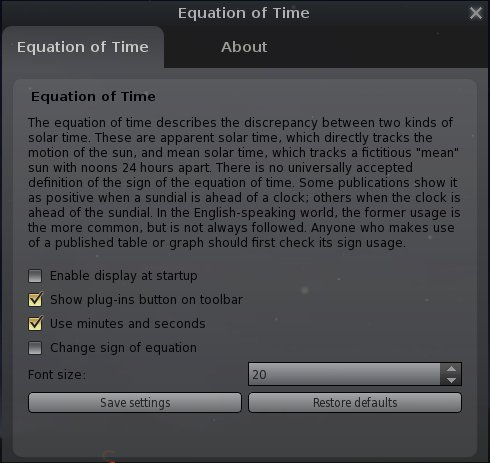
\includegraphics[width=\textwidth]{EquationOfTime-plugin.jpg}
%\label{fig:EqOfTime}
%\caption{Interface of Equation of Time plugin}
%\end{figure}

\begin{figure}[h]\centering
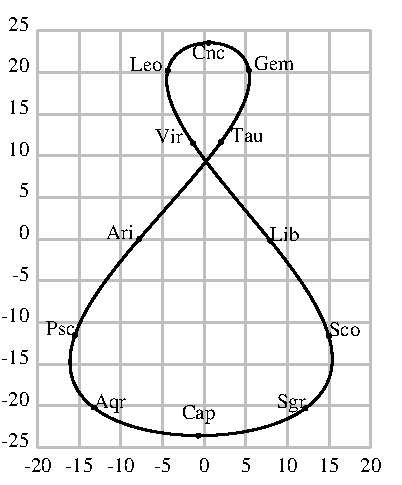
\includegraphics[width=.3\textwidth]{GZ_analemma_p1000}
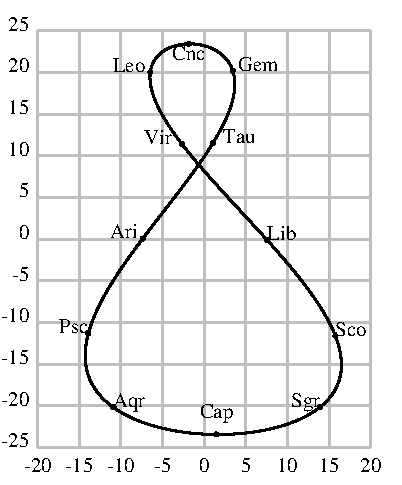
\includegraphics[width=.3\textwidth]{GZ_analemma_p2000}
\label{fig:EqOfTime}
\caption{Figure-8 plots for Equation of Time, for years 1000 (left)
  and 2000 (right). These plots, often found on sundials, link solar
  declination (vertical axis) and its deviation at mean noon from the
  meridian, in minutes. Labeled dots indicate when the sun entered the
  respective Zodiacal sign (30\degree section of the
  ecliptic). Figures by Georg Zotti.}
\end{figure}


\noindent The Equation of Time plugin shows the solution of the equation of time. % (Fig.~\ref{fig:EqOfTime}).
This describes the discrepancy between two kinds of
solar time:
\begin{description}
\item[Apparent solar time] directly tracks the motion of the sun. Most sundials show this time.
\item[Mean solar time] tracks a fictitious ``mean'' sun with noons 24 hours apart. 
\end{description}

There is no universally accepted definition of the sign of the
equation of time. Some publications show it as positive when a sundial
is ahead of a clock; others when the clock is ahead of the sundial. In
the English-speaking world, the former usage is the more common, but
is not always followed. Anyone who makes use of a published table or
graph should first check its sign usage.

If enabled (see section~\ref{sec:Plugins:EnablingPlugins}), click on
the Equation of Time button \guibutton{0.6}{bt_EquationOfTime_72dpi}
on the bottom toolbar to display the value for the equation of time on
top of the screen.


\subsection{Section \big[EquationOfTime\big] in config.ini file}
\label{sec:plugins:EquationOfTime:config}

You can edit \file{config.ini} file by yourself for changes of the
settings for the Equation of Time plugin -- just make it carefully!

\begin{longtabu} to \textwidth {l|l|X}\toprule
\emph{ID}            & \emph{Type} & \emph{Description}\\\midrule
enable\_at\_startup  & bool & Display solution of the equation of time at startup of the planetarium\\\midrule
flag\_use\_ms\_format & bool & Set format for the displayed solution - minutes and seconds and decimal minutes\\\midrule
flag\_use\_inverted\_value & bool & Change sign of the equation of time \\\midrule
flag\_show\_button & bool & Enable displaying plugin button on the bottom toolbar\\\midrule
text\_color & R,G,B & Color of font for the displayed solution of the equation of time\\\midrule
font\_size & int & Font size for the displayed solution of the equation of time \\\bottomrule
\end{longtabu}



\newpage

\section{Field of View Plugin}
\label{sec:plugins:FieldOfView}

\begin{figure}[ht]\centering
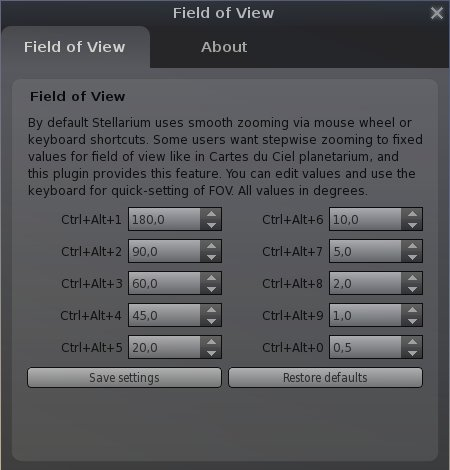
\includegraphics[trim=0 55 0 0,clip,width=.55\textwidth]{FOV-plugin.jpg}
\label{fig:plugins:FieldOfView}
\caption{Configuration dialog of Field of View plugin}
\end{figure}

\noindent By default Stellarium uses smooth zooming via mouse wheel or
keyboard shortcuts. Some users may want stepwise zooming to fixed
values for field of view like in the \program{Cartes du
  Ciel}\footnote{SkyChart / Cartes du Ciel planetarium:
  \url{http://www.ap-i.net/skychart/en/start}} planetarium program,
and this plugin provides this feature. You can edit values and use the
keyboard for quick-setting of FOV. All values in degrees.

%\section{Using the Field of View plugin}
%\label{sec:plugins:FieldOfView:using}

\begin{enumerate}
\item Enable the tool by configuring it to ``Load at startup''.
\item Press shortkeys for quick changes of FOV.
\end{enumerate}

\subsection{Section \big[FOV\big] in config.ini file}
\label{sec:plugins:FieldOfView:config}

You can configure the plugin with its dialog (Fig.~\ref{fig:plugins:FieldOfView}) or edit
\file{config.ini} file by yourself for changes of the settings for the
Field of View plugin -- just make it carefully!

\begin{longtabu} to \textwidth {l|l|r|X}\toprule
\emph{ID} & \emph{Type} & \emph{Default} & \emph{Description}\\\midrule
fov\_quick\_0  & float & 0.5& Value of FOV for the shortcut \key{\ctrl+\Alt+0} \\\midrule
fov\_quick\_1  & float &180 & Value of FOV for the shortcut \key{\ctrl+\Alt+1} \\\midrule
fov\_quick\_2  & float & 90 & Value of FOV for the shortcut \key{\ctrl+\Alt+2} \\\midrule
fov\_quick\_3  & float & 60 & Value of FOV for the shortcut \key{\ctrl+\Alt+3} \\\midrule
fov\_quick\_4  & float & 45 & Value of FOV for the shortcut \key{\ctrl+\Alt+4} \\\midrule
fov\_quick\_5  & float & 20 & Value of FOV for the shortcut \key{\ctrl+\Alt+5} \\\midrule
fov\_quick\_6  & float & 10 & Value of FOV for the shortcut \key{\ctrl+\Alt+6} \\\midrule
fov\_quick\_7  & float &  5 & Value of FOV for the shortcut \key{\ctrl+\Alt+7} \\\midrule
fov\_quick\_8  & float &  2 & Value of FOV for the shortcut \key{\ctrl+\Alt+8} \\\midrule
fov\_quick\_9  & float &  1 & Value of FOV for the shortcut \key{\ctrl+\Alt+9} \\\bottomrule
\end{longtabu}

\newpage

\section{Pointer Coordinates Plugin}
\label{sec:plugins:PointerCoordinates}


\begin{figure}[th]\centering
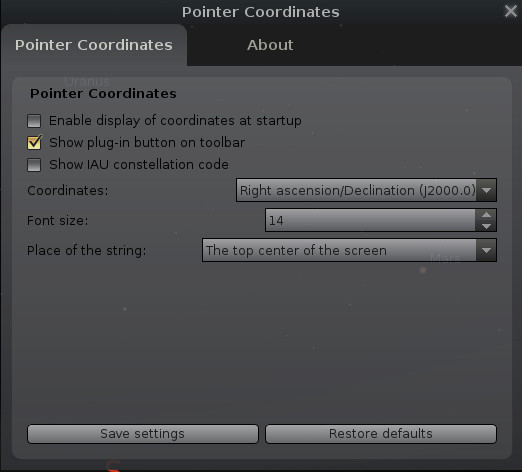
\includegraphics[trim=0 140 0 0,clip,width=.9\textwidth]{PointerCoordinates-plugin.jpg}
\label{fig:PointerCoordinates}
\caption{Interface of Pointer Coordinates plugin}
\end{figure}

\noindent The Pointer Coordinates plugin shows the coordinates of the mouse pointer.
If enabled, click on the plugin button \guibutton{0.6}{bt_PointerCoordinates_Off} on the bottom toolbar to display the coordinates of the mouse pointer.

\subsection{Section \big[PointerCoordinates\big] in config.ini file}
\label{sec:plugins:PointerCoordinates:config}

You can edit \file{config.ini} file by yourself for changes of the
settings for the Pointer Coordinates plugin -- just make it carefully!

\begin{longtabu} to \textwidth {l|l|X}\toprule
\emph{ID}            & \emph{Type} & \emph{Description}\\\midrule
enable\_at\_startup  & bool & Enable displaying coordinates of the mouse pointer at startup of the plugin\\\midrule
flag\_show\_button   & bool & Enable showing the button of the plugin on bottom toolbar\\\midrule
text\_color          & R,G,B & Color for text with coordinates of the mouse pointer \\\midrule
font\_size           & int & Font size for the displayed coordinates of the mouse pointer \\\midrule
current\_displaying\_place  & string & Specifies the place of displaying coordinates of the mouse pointer. \textit{Possible values}: \keymap{TopRight}, \keymap{TopCenter}, \keymap{RightBottomCorner}, \keymap{Custom}. \textit{Default value}: \keymap{TopRight}. \\\midrule
current\_coordinate\_system & string & Specifies the coordinate system. \textit{Possible values}: \keymap{RaDecJ2000}, \keymap{RaDec}, \keymap{HourAngle}, \keymap{Ecliptic}, \keymap{AltAzi}, \keymap{Galactic}. \textit{Default value}: \keymap{RaDecJ2000}. \\\midrule
custom\_coordinates  & int,int & Specifies the screen coordinates of the custom place for displaying coordinates of the mouse pointer \\\bottomrule
\end{longtabu}




\newpage

\section{Text User Interface}
\label{sec:plugins:TextUserInterface}

%\url{http://porpoisehead.net/images/plugin-tui.jpg}

This plugin re-implements the ``TUI'' of the pre-0.10 versions of
Stellarium, an unobtrusive menu used primarily by planetarium system
operators to change settings, run scripts and so on.

Given that color configuration for lines and texts cannot be found
elsewhere, an interesting part for general use (at least for extended
configuration sessions) is the way to interactively select colors in
this menu.

A full list of the commands for the TUI plugin is
given in section~\ref{sec:plugins:TUI:commands}. 

\subsection{Using the Text User Interface}
\label{sec:plugins:TUI:using}

\begin{enumerate}
\item Activate the text menu using the \key{\Alt+T} key.\footnote{This
    used to be hard-coded to \key{M} before version 0.15, but
    \key{\Alt+T} is better to remember as it runs parallel with
    \key{\ctrl+T} for switching the GUI panels, and frees up \key{M}
    for the Milky Way. The \key{\Alt+T} keybinding is hardcoded, i.e.,
    cannot be reconfigured by the user, and should not be used for
    another function.}
\item
  Navigate the menu using the cursors keys.
\item
  To edit a value, press the right cursor until the value you wish to
  change it highlighted with \textgreater{} and \textless{} marks, e.g.\
  \textgreater{}3.142\textless{}. Then press the cursor keys \keys{\arrowkeyup} and \keys{\arrowkeydown} to
  change the value. You may also type in a new value with the other keys
  on the keyboard.
\end{enumerate}

%% List complete as of 2016-04-26. 

\subsection{TUI Commands}
\label{sec:plugins:TUI:commands}
\begin{longtabu} to \textwidth {l|l|X}
\toprule
1   & Location & (menu group)\\\midrule
1.1 & Latitude & Set the latitude of the observer in degrees\\\midrule
1.2 & Longitude & Set the longitude of the observer in degrees\\\midrule
1.3 & Altitude & Set the altitude of the observer in meters\\\midrule
1.4 & Solar System Body & Select the solar system body on which the observer is\\\midrule
2   & Set Time & (menu group)\\\midrule
2.1 & Current date/time & Set the time and date for which Stellarium will generate the view\\\midrule
%2.2 & Set Time Zone & Set the time zone. Zones are split into continent or region, and then by city or province\\\midrule
%2.3 & Days keys & The setting ``Calendar'' makes the \key{-}, \key{=}, \key{[}, \key{]} keys change the date value by calendar days (multiples of 24 hours). 
%                  The setting ``Sidereal day'' changes these keys to change the date by sidereal days\\\midrule
2.2 & Set Time Zone & (disabled in 0.15)\\
2.3 & Days keys & (disabled in 0.15)\\
2.4 & Startup date/time preset & Select the time which Stellarium starts with (if the ``Sky Time At Start-up'' setting is ``Preset Time''\\\midrule
2.5 & Startup date and time & The setting ``system'' sets Stellarium's time to the computer clock when Stellarium runs. 
                                 The setting ``preset'' selects a time set in menu item ``2.4 - Startup date/time preset''\\\midrule
2.6 & Date Display Format & Change how Stellarium formats date values. ``system\_default'' takes the format from the computer settings, 
                            or it is possible to select ``yyyymmdd'', ``ddmmyyyy'' or ``mmddyyyy'' modes\\\midrule
2.7 & Time Display Format & Change how Stellarium formats time values. ``system\_default'' takes the format from the computer settings, 
                            or it is possible to select ``24h'' or ``12h'' clock modes\\\midrule
3    & General & (menu group)\\\midrule
3.1  & Starlore & Select the sky culture to use (changes constellation lines, names, artwork)\\\midrule
3.2  & Sky Language & Change the language used to describe objects in the sky\\\midrule
3.3  & App Language & Change the application language (used in GUIs) \\\midrule
4    & Stars & (menu group)\\\midrule
4.1  & Show stars & Turn on/off star rendering\\\midrule
4.2  & Relative Scale & Change the relative brightness of the stars. Larger values make bright stars much larger.\\\midrule
4.3  & Absolute Scale & Change the absolute brightness of the stars. Large values show more stars. Leave at 1 for realistic views. \\\midrule
4.4  & Twinkle & Sets how strong the star twinkling effect is - zero is off, the higher the value the more the stars will twinkle.\\\midrule
5    & Colors & (menu group)\\\midrule
5.1  & Constellation lines         & Changes the colour of the constellation lines\\\midrule
5.2  & Constellation labels        & Changes the colour of the labels used to name stars\\\midrule
5.3  & Art brightness              & Changes the brightness of the constellation art\\\midrule
5.4  & Constellation boundaries    & Changes the colour of the constellation boundary lines\\\midrule
5.5  & Cardinal points             & Changes the colour of the cardinal points markers\\\midrule
5.6  & Planet labels               & Changes the colour of the labels for planets\\\midrule
5.7  & Planet orbits               & Changes the colour of the orbital guide lines for planets\\\midrule
5.8  & Planet trails               & Changes the colour of the planet trails lines\\\midrule
5.9  & Meridian Line               & Changes the colour of the meridian line\\\midrule
5.10 & Azimuthal Grid              & Changes the colour of the lines and labels for the azimuthal grid\\\midrule
5.11 & Equatorial Grid             & Changes the colour of the lines and labels for the equatorial grid\\\midrule
5.12 & Equatorial J2000 Grid       & Changes the colour of the lines and labels for the equatorial J2000.0 grid\\\midrule
5.13 & Equator Line                & Changes the colour of the equator line\\\midrule
5.14 & Ecliptic Line               & Changes the colour of the ecliptic line\\\midrule
5.15 & Ecliptic Line (J2000)       & Changes the colour of the J2000 ecliptic line\\\midrule
5.16 & Nebula names                & Changes the colour of the labels for nebulae\\\midrule
5.17 & Nebula hints                & Changes the colour of the circles used to denote the positions of unspecified nebulae\\\midrule
5.18 & Galaxy hints                & Changes the colour of the ellipses used to denote the positions of galaxies\\\midrule
5.19 & Bright nebula hints         & Changes the colour of the squares used to denote the positions of bright nebulae\\\midrule
5.20 & Dark nebula hints           & Changes the colour of the squares used to denote the positions of dark nebulae\\\midrule
5.21 & Clusters hints              & Changes the colour of the symbols used to denote the positions of clusters\\\midrule
5.22 & Horizon line                & Changes the colour of the horizon line\\\midrule
5.23 & Galactic grid               & Changes the colour of the galactic grid\\\midrule
5.24 & Galactic equator line       & Changes the colour of the galactic equator line\\\midrule
5.25 & Opposition/conjunction longitude line & Changes the colour of the opposition/conjunction line\\\midrule
6   & Effects & (menu group)\\\midrule
6.1 & Light Pollution & Changes the intensity of the light pollution (see Appendix~\ref{ch:BortleScale} Bortle Scale index)\\\midrule
6.2 & Landscape   & Select the landscape which Stellarium draws when ground drawing is enabled. Press \key{\return} to activate.\\\midrule
6.3 & Setting Landscape Sets Location & If ``Yes'' then changing the landscape will move the observer location to the location for that landscape (if one is known). 
                                        Setting this to ``No'' means the observer location is not modified when the landscape is changed.\\\midrule
6.4 & Auto zoom out returns to initial \ldots view & Changes the behaviour when zooming out from a selected object.
                    When set to ``Off'', selected object will stay in center.
                    When set to ``On'', view will return to startup view. \\\midrule
6.5 & Zoom Duration & Sets the time for zoom operations to take (in seconds)\\\midrule
6.6 & Milky Way intensity & Changes the brightness of the Milky Way\\\midrule
6.7 & Zodiacal light intensity & Changes the brightness of the Zodiacal light\\\midrule
%6.6 & Nebula label frequency & Changes the magnitude limit for labelling of nebulae\\\midrule
%6.6 & Nebula label frequency & (not active) \\\midrule
%6.8 & Cursor Timeout & Sets the number of seconds of mouse inactivity before the cursor vanishes\\\midrule
7 & Scripts & (menu group)\\\midrule
7.1 & Run local script       & Run a script from the scripts sub-directory of the User Directory or Installation Directory 
                               (see section~\ref{sec:FilesAndDirectories} (Files and Directories))\\\midrule
7.1 & Stop running script    & Stop execution of a currently running script \\\midrule
%7.2 & CD/DVD Script          & Run a script from a CD or DVD (only used in planetarium set-ups)\\\midrule
8   & Administration             & (menu group)\\\midrule
8.1 & Load default configuration & Reset all settings according to the main configuration file\\\midrule
8.2 & Save current configuration & Save the current settings to the main configuration file\\\midrule
8.3 & Shutdown                   & Emits a command configured in \\\midrule
\end{longtabu}


\subsection{Section \big[tui\big] in config.ini file}
\label{sec:plugins:TUI:config}

The section in \file{config.ini} for this plugin is named only \texttt{[tui]} for historical reasons. As always, be careful when editing!

\begin{longtabu} to \textwidth {l|l|X}\toprule
\emph{ID}            & \emph{Type} & \emph{Description}\\\midrule
tui\_font\_color     & R,G,B & Font color for TUI text \\\midrule
tui\_font\_size      & int   & Font size for the TUI \\\midrule
flag\_show\_gravity\_ui           &bool&Bend menu text around the screen center. 
                                        May be useful in planetarium setups, and should then be used together with ``Disc viewport'' 
                                        in the configuration menu (see~\ref{sec:gui:configuration:tools}). \\\midrule
flag\_show\_tui\_datetime         &bool&Show date and time in lower center.\\\midrule
flag\_show\_tui\_short\_obj\_info &bool&Show some object info in lower right, or (in planetarium setups with ``Disc viewport'' active,) wrapped along the outer circle border. \\\midrule
admin\_shutdown\_cmd              &string& executable command to shutdown your system. Best used on Linux or Mac systems. E.g.\ \texttt{shutdown -h now}\\\bottomrule
\end{longtabu}



\newpage
\section{Remote Control}
\label{sec:plugin:RemoteControl}

[This will come as user documentation from SoCiS2015 work]


% \newpage
% \section{D-Bus Interface}
% \label{sec:plugin:DBus}
% 
% [This may come as user documentation from SoCiS2016 (?) work]


\newpage

\section{Solar System Editor Plugin}
\label{sec:plugins:SolarSystemEditor}

Stellarium stores its data (orbital elements and other details) about
solar system objects (planets, their moons, minor bodies) in the file
\file{data/ssystem.ini}. The file will be taken from the user data
directory if it also exists there, which means, users can add minor
planets or comets as they become observable by editing this file.


This plugin provides a window to the Minor Planet Center (MPC) where the
latest Solar System information can be found. When this plugin is
loaded (see section~\ref{sec:Plugins:EnablingPlugins}) the first tab
allows to import, export or reset your \file{ssystem.ini}.

The second tab lists all currently loaded objects.  It is recommended
to remove old entries of last year's comets if you don't need them any
longer.
If you have a very weak computer, you may want to reduce the number of
minor bodies (and maybe even planetary moons) to improve performance.

On this tab, you find the option to connect to the MPC and download current orbital elements. 


\newpage

\section{Timezone Configuration Plugin}
\label{sec:plugins:Timezones}


\begin{figure}[h]\centering
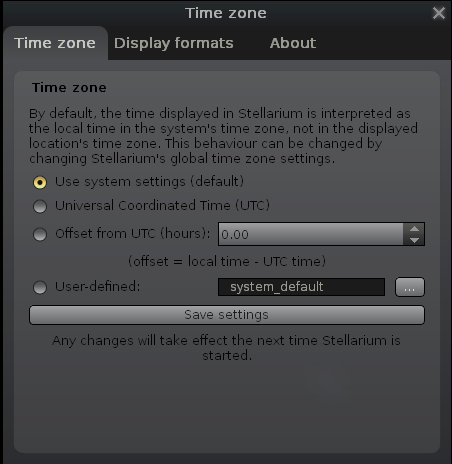
\includegraphics[width=.9\textwidth]{Timezone}
\label{fig:plugins:Timezones}
\caption{Interface of the TimeZone Configuration Plugin}
\end{figure}


\noindent After installation, Stellarium uses the timezone configured in the
computer's operating system. This may have unwanted consequences,
e.g.\ when you want to check the sky for a location on another
continent. You may set location in the location panel (see
\ref{sec:gui:location}), but the time will not be the zone time of
this location but still zone time of your computer!

Another effect of our civilisation that sometimes brings unwanted side
effects concerns daylight saving time (DST): When you run a timelapse
with 1-day intervals, you will see what appear to be wrong jumps on
the days when DST is switched (e.g., end of March/end of October, but
rules evolve over time and regions). You may want to keep a single
time zone without DST for such simulations.


If enabled (see section~\ref{sec:Plugins:EnablingPlugins}), you can
choose to use your timezone (default), or plain Universal Coordinated
Time (UTC) (equivalent to what used to be called Greenwich Mean Time
GMT), or select a time zone (in steps of 15 minutes). 

Note that you must exit and restart Stellarium to activate the new
timezone, so jumping from location to location on Earth and showing
correct zone time is not possible.

%% TODO: Obviously, we should adapt our TZ handling to make this
%% possible! Store TZ in location list, and suggest/guess TZ from
%% longitude of map-clicked location.


%%% Local Variables: 
%%% mode: latex
%%% TeX-master: "guide"
%%% End: 

